%!TEX program = xelatex
% 完整编译: xelatex -> bibtex -> xelatex -> xelatex
\documentclass[lang=cn,11pt,a4paper,cite=super,AutoFakeBold,chinesefont=founder]{elegantpaper}

\title{基于CiteSpace探讨近10年推拿治疗颈椎病的研究趋势}
\author{051851601\ 崔暖}
% \institute{(湖北民族大学\ 医学部,湖北恩施\ 445000)\vspace*{-3em}}
\institute{\vspace*{-3em}}
\date{}

\usepackage{ctex}
\setCJKfamilyfont{song}{SimSun}

\usepackage{array}
\newcommand{\ccr}[1]{\makecell{{\color{#1}\rule{1cm}{1cm}}}}
\usepackage{siunitx}
\usepackage[version=4]{mhchem}		% 化学公式
\usepackage{makecell}				%表格内换行

\newcommand{\cnabs}{\noindent{\small \textsf{摘要}}\quad}
\newcommand{\cnkys}{\noindent{\small \textsf{关键词}}\quad}
\newcommand{\enabs}{\noindent{\textbf{Abstract}\quad}}
\newcommand{\enkys}{\noindent{\textbf{Key Words}\quad}}

\renewcommand{\abstractname}{}

% 正文区
\begin{document}
\maketitle

% 摘要
\begin{onecolabstract}
\cnabs
目的:分析国内近10年推拿治疗颈椎病的研究现状和发展趋势。
方法:以CNKI数据库近10年的文献作为数据来源,使用CiteSpace软件作为工具,通过合作网络、关键词聚类、关键词共现等分析研究作者、研究热点与未来趋势。
结果:共纳入2312篇文献进行分析;近10年的发文量总体呈增长趋势;合作关系网络中影响力最大的是孙武权的团队;文献关键词可聚类为颈椎病、推拿手法、临床疗效、血流动力学等11个类型。有推拿疗法、综合疗法、牵引术、功能锻炼、血流动力学等15个突现关键词。
结论:作者及各研究主体之间应该加强相互间的合作, 规范相关术语, 构建更大规模的平台, 为相关研究的进一步深入进展提供更有利的条件。

\cnkys
颈椎病; 推拿疗法; CiteSpace; 知识图谱; 可视化分析
\end{onecolabstract}

% 以“推拿”、“颈椎病”为主题词在中国知网中检索,时间限定在2011/1/1 -- 2021/11/10,共检索出3053条相关文献,经过筛选,剩余2316条相关文献,导入CiteSpace并进行格式转化,成功识别出2312条题录。

% 356字
颈椎病是骨科常见的一种退行性病变综合征,包括颈椎间盘脱出、颈椎骨关节炎等多种疾病。颈椎病常由慢性劳损、骨质增生、颈椎管狭窄等多种因素引起,临床表现为项背酸痛、四肢乏力、手麻、行走困难等症状,常并发吞咽障碍、视物不清、失眠、恶心呕吐等疾病。对于颈椎病的治疗,现代医学常采用药物镇静镇痛、牵引、手术等方案,但这些方法在适宜人群、患者感受和预后等方面均有不足,一定程度上限制了其疗效和应用面。随着中医理疗观念的广泛传播,推拿治疗颈椎病的方法日益受到重视,因其疗效可观、简便易行、适用面广,一度成为临床研究的重点。然而目前尚无研究对这一领域的相关文献进行脉络梳理,故为了更好地展现当前推拿治疗颈椎病的研究热点与趋势,本研究借助CiteSpace软件,对近10年来的相关文献进行可视化分析,以期为进一步的临床研究提供参考。

\section{资料与方法}

\subsection{数据来源}

选用中国知网(CNKI)数据库,以“推拿”、“颈椎病”等关键词为主题进行检索,时间范围控制在2011年1月1日 -- 2021年11月10日。检索完成后进行文献筛选,排除个人经验介绍、会议通知、学位论文、征稿通知、报刊广告和其他无关“推拿治疗颈椎病”的文献,确保纳入的文献符合本研究的需要。

\subsection{数据转换}

筛选完所需的文献后,将其以Refwork格式将题录导出,包括题名、作者、机构、摘要、关键词、发表年份、期刊名等信息,文件以“download\_XX.txt”格式命名。将题录文件导入CiteSpace 5.8.R1,对其进行标准化处理,留存备用。

\subsection{分析方法}

使用CiteSpace 5.8.R1对标准化后的数据进行可视化分析,通过绘制作者共现图、机构合作图、关键词共现图、关键词聚类图和关键词时间线等可视化图谱,展现该领域近10年的研究热点与未来发展趋势。

\section{结果}

\subsection{文献检索结果}

在中国知网中共检索出3053篇文献,剔除了会议、学位、报刊等无关文献737篇,并导入CiteSpace软件进行转换处理,最终纳入2312篇相关文献进行分析。    % 文献发表年份统计流程:题录 -> 正则表达式 -> Excel -> R语言

\subsection{年发文量分析} % 图1

本研究通过分析年度发文量的变化,从整体把握推拿治疗颈椎病的研究动态。将纳入的2312篇文献按照发表年份排列,统计各年的发文量,根据图\ref{figure:1}可知,近10年的发文趋势可分为以下两个阶段:

(1) 2011年 -- 2019年:这个时期的各年的发文量差异较大,增减幅度明显,但整体呈增长态势,且于2019年达近10年发文量之最(264篇)。在此阶段,学者们尝试从多方面阐释推拿治疗颈椎病的作用机制,并将理论研究的成果运用于临床。但由于此时科技水平受限,各项基础研究进入了瓶颈期,且现代医学对中医推拿的冲击持续存在,故文献数量的增长不够稳定。

(2) 2020年 -- 2021年:这个时期中,由于新冠肺炎疫情的影响,大量的基础实验和临床研究不能正常开展,导致发文量逐年降低。但这不代表研究热点的消失,待消除疫情的影响,研究于发文量仍有回升的可能。

\begin{figure}[htbp]
  \centering
  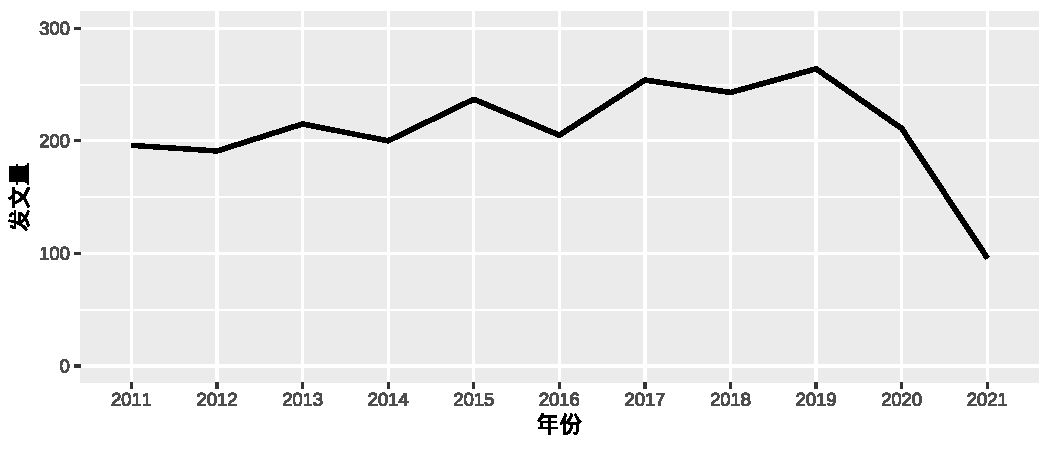
\includegraphics[width=0.8\textwidth]{figure/年发文量.pdf}
  \caption{近10年发文量变化趋势}
  \label{figure:1}
\end{figure}

\subsection{作者共现分析} % 图2

在CiteSpace中,将节点类型(Node Type)设置为作者(Author),分析各作者的发文量,以及不同作者之间的合作关系。图\ref{figure:2}中各节点代表不同的作者,节点半径越大表示作者发文量越多,节点间连线代表不同作者的联合发文情况。发文量前五的作者依次为房敏(18篇)、孙武权(13篇)、朱清广(13篇)、沈国权(9篇)、陈水金(8篇)。由图2可见,共形成了4个研究团体,其中以孙武权为中心的团队发文量最多,此团队的研究内容主要为筋骨评估、筋骨失衡和脊柱微调手法等。这些研究团队只在内部形成小范围的合作关系,缺少团队之间的合作交流,未来应加强各个团队之间的联系来共同发展。

\begin{figure}[!ht]
  \centering
  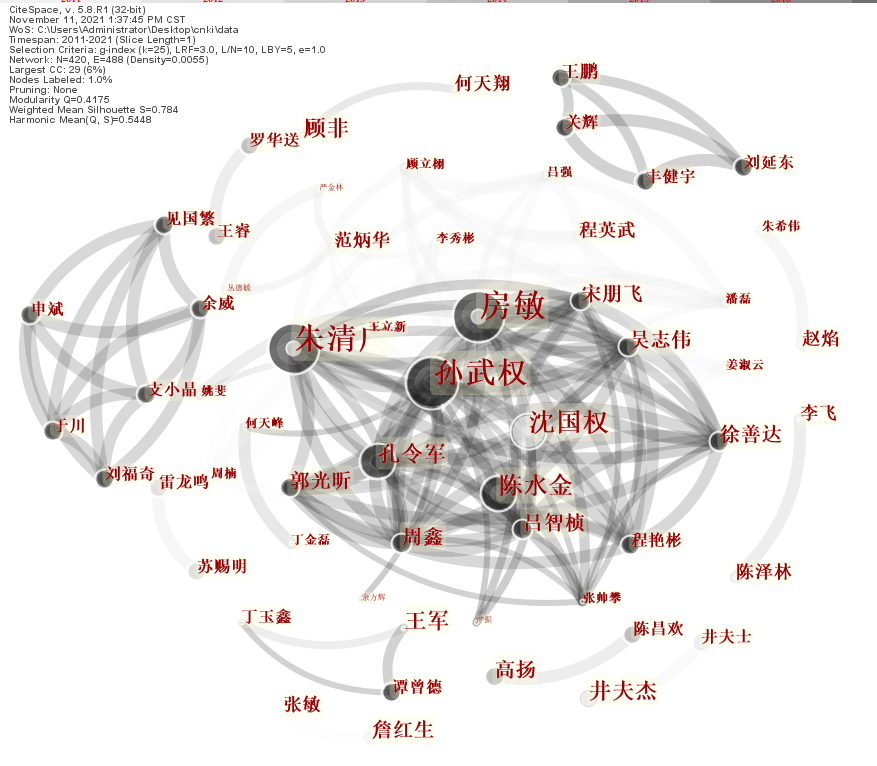
\includegraphics[width=0.6\textwidth]{figure/作者共现.png}
  \caption{作者共现知识图谱}
  \label{figure:2}
\end{figure}

\subsection{关键词共现分析} % 图3 表1

将节点类型设置为关键词(KeyWords),阈值设置为10得出关键词共现图,见图\ref{figure:3}。图中节点越大,代表该关键词出现的频数越高,越受研究者关注。具有紫色外圈的节点,表示该关键词的中心性较大,在图谱中发挥着桥梁作用。该图谱中,共有545个节点,1626条连线,网络密度为0.011。截取中心性大于0.01的关键词生成关键词频次表,由表\ref{tabular:1}可见,高频关键词包括疾病类型(颈椎病、神经根型颈椎病、椎动脉型颈椎病、颈型颈椎病),治疗方法(推拿手法、针灸推拿、推拿疗法),以及疗效评估(临床观察、临床效果、疗效观察)。这些关键词代表目前该研究领域的热点话题:以推拿为主,并结合针灸、方药等其他治法,研究各种类型颈椎病的治疗,并使用多种手段评估疗效,促进推拿治法治则进一步完善。

\begin{figure}[!ht]
  \centering
  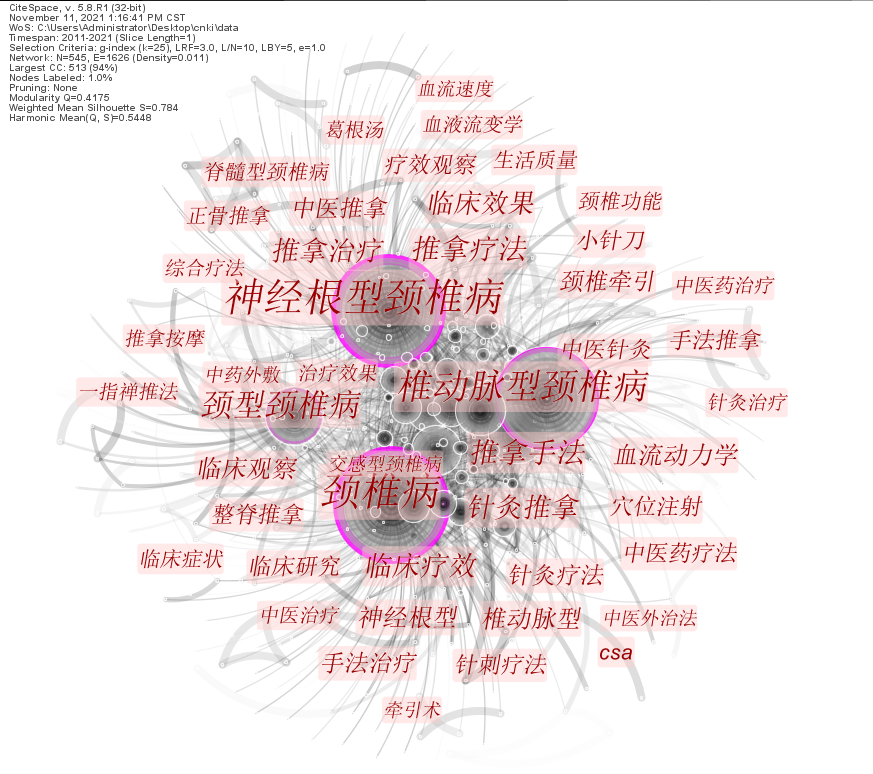
\includegraphics[width=0.6\textwidth]{figure/关键词共现.png}
  \caption{关键词共现知识图谱}
  \label{figure:3}
\end{figure}

\begin{table}[!ht]
\caption{高频关键词$(\text{Centrality} > 0.01)$}
  \centering
  \begin{tabular}{*4{c}}
  \toprule
  频次  & 中心性  & 年份   & 关键词     \\
  \midrule
  723 & 0.76 & 2011 & 颈椎病     \\
  648 & 0.71 & 2011 & 神经根型颈椎病 \\
  520 & 0.33 & 2011 & 椎动脉型颈椎病 \\
  143 & 0.16 & 2011 & 颈型颈椎病   \\
  142 & 0.05 & 2011 & 推拿手法    \\
  110 & 0.03 & 2011 & 针灸推拿    \\
  101 & 0.06 & 2011 & 推拿疗法    \\
  85  & 0.04 & 2011 & 临床疗效    \\
  70  & 0.04 & 2011 & 推拿治疗    \\
  49  & 0.02 & 2011 & 临床观察    \\
  49  & 0.02 & 2012 & 临床效果    \\
  32  & 0.03 & 2015 & 血流动力学   \\
  30  & 0.02 & 2011 & 疗效观察    \\
  18  & 0.02 & 2011 & 手法治疗    \\
  \bottomrule
  \label{tabular:1}
  \end{tabular}
\end{table}

\subsection{关键词聚类分析} % 图4 表2

关键词聚类是通过对文献主题高度概括的核心关键词进行聚类分析,可以帮助迅速了解该研究领域的分布情况及研究前沿。在关键词共现的基础上,选择“Keyword”,对主要关键词进行自动聚类,由图\ref{figure:4}所示,共得出11个聚类。CiteSpace使用模块值$Q$和平均轮廓值$S$作为判断绘制效果的依据,如果$Q>0.3$,说明图谱结构合理,如果$S>0.5$,说明网络的同质性合理,如果$S>0.7$,则说明聚类结果是可信的。% 此处引用:陈悦, 陈超美, 刘则渊, 等.CiteSpace知识图谱的方法论功能[J].科学学研究, 2015, 33(2): 242-253.
本研究结果中,$Q=0.4175(>0.3)$,$S=0.784(>0.7)$,表明该聚类图谱的绘制效果是比较可信的,各聚类交叉重叠,说明聚类间联系密切。

为了更好地把握研究热点,可以将聚类结果分为三大领域:

(1) 对不同疾病类型的研究:对神经根型颈椎病的研究(\#0);对颈椎病的研究(\#1);对椎动脉型颈椎病的研究(\#2);对颈型颈椎病的研究(\#4)。

(2) 对各种治法治则的研究:对针灸结合推拿治疗的研究(\#3);对单用推拿治疗的研究(\#5、\#6);对颈椎牵引的研究(\#8)。

(3) 对评估临床疗效的研究:对临床疗效的研究(\#7);对随机平行对照试验的研究(\#9);对中医证候积分的研究(\#10)。

% 归纳后通过进一步分析各聚类 silhouette 值、 平均引用年份与 size 值, 发现各聚类 silhouette 较高 (≥0.825 ) , 文献关键程度高, 聚类 1、 聚类 2、 聚类 3、 聚类4 研究热度高, 聚类 10 引用年份较近, 说明子午流注针法的热点主题为临床研究与基础研究, 临床研究关注度最高, 研究量增长快, 逐渐由单一疗法向多疗法、 多疾病、 多领域拓宽, 其治疗理疗思想正在影响更多疗法。

% 的silhouette值较高$(\ge 0.68)

\begin{figure}[!ht]
  \centering
  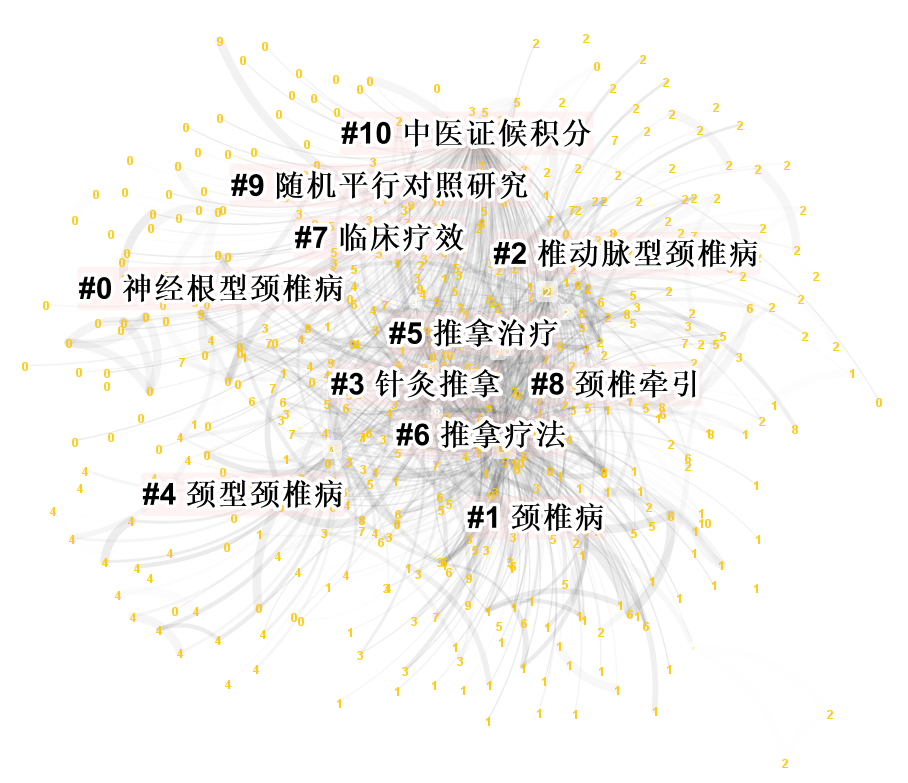
\includegraphics[width=0.6\textwidth]{figure/关键词聚类.png}
  \caption{关键词聚类知识图谱}
  \label{figure:4}
\end{figure}

通过进一步分析各聚类silhouette值、size值和平均引用年份,发现\#0、\#1、\#2和\#3的研究热度最高,发文量最大,文献关联程度强(见表\ref{tabular:2})。说明对于推拿治疗颈椎病的研究,各学者更多地关注疾病本身,研究颈椎病发生发展的各种影响因素,为后续的临床治疗环节提供依据。

\begin{table}[!ht]
  \caption{高频关键词$(\text{Centrality} > 0.01)$}
    \centering
    \begin{tabular}{*4{c}}
    \toprule
    Cluster ID & Size & Silhouette & mean(Citee Year) \\
    \midrule
    0          & 99   & 0.68       & 2015             \\
    1          & 87   & 0.778      & 2014             \\
    2          & 77   & 0.803      & 2016             \\
    3          & 54   & 0.804      & 2015             \\
    \bottomrule
    \label{tabular:2}
    \end{tabular}
  \end{table}


\subsection{研究趋势分析} % 图5

研究前沿代表了相关领域当前的研究趋势, 而关键词的突现率反映了一段时间内受到广泛关注, 容易成为研究领域的前沿主题。使用CiteSpace软件绘制关键词突现图, 展示不同时段突现词的变化, 可探知推拿治疗颈椎病在当前的研究趋势。

% 在图 6 中, “失眠”“穴位贴敷”“便秘”“脑卒中” 四个突现词激增最为显著。归纳提炼文献, 发现各突现词均属于子午流注针法临床疗效观察。1 “失眠” 的突现强度最高, 为 10.0731, 自 2011 年起主要为原发性失眠的研究, 后逐渐扩展为继发性失眠的研究, 由单一的时间针刺研究向时间针灸联合其他中医疗法的临床研究转变; 2 “穴位贴敷” 和 “便秘” 突现强度分别是9.2987、 7.8433, 两个突现词常共同出现于研究文献中, 主要为择时选穴与穴位贴敷法的结合运用; 3 “脑卒中” 突现强度为 5.3881, 脑卒中属针灸优势病种, 研究较早, 现主要研究为脑卒中引起的并发症如睡眠倒错、便秘。子午流注针法的研究前沿主要为失眠、 便秘、 脑卒中三种疾病的临床疗效观察, 且逐渐细致深化, 最新研究前沿是子午流注取穴思想指导下的各疗法新用。

由图\ref{figure:5}可见,“葛根汤”、“治疗效果”、“颈椎功能”、“血流动力学”4个突现词激增最为显著。归纳文献后发现,各突显词均属于推拿治疗颈椎病的相关研究概括。

(1) “葛根汤”的突现强度为3.38,自2017年起有葛根汤联合推拿治疗颈椎病的研究。

(2) “治疗效果”的突显强度为3.91,自2018年起,临床治疗的疗效评估受到重视,且与“葛根汤”的突现时间接近,提示该阶段尝试将多种治法相互比较,评估出最适合的方法。

(3) “颈椎功能”和“血流动力学”的突现时间相同,均为2019年,突显强度分别为5.72、4.07。该阶段的研究热点开始由临床治疗转向基础研究,联合现代医学技术,在微观层面探究颈椎病的发生发展机制,以期寻找临床治疗的突破口。

\begin{figure}[!ht]
  \centering
  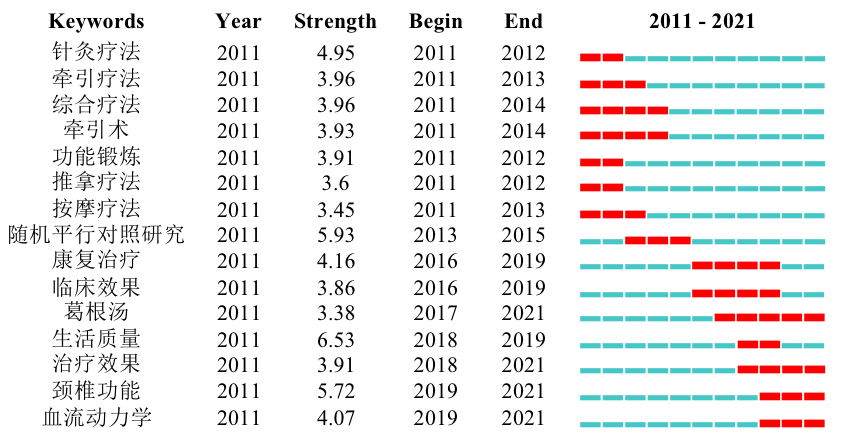
\includegraphics[width=0.6\textwidth]{figure/关键词突现.png}
  \caption{关键词突现知识图谱}
  \label{figure:5}
\end{figure}

\section{结论}

颈椎病在中医里归属“颈肩痛”、“筋病”范畴,多由体弱气虚、感受外邪、气血亏虚、气滞血瘀等因素引起。推拿有舒经活络、放松肌肉、加快血液循环的功效,对颈椎病有较好的疗效。本研究利用CiteSpace软件,对中国知网上近10年关于推拿治疗颈椎病的2312篇文献进行可视化,分析了年发文量、作者联合发文情况、现阶段研究内容和未来发展趋势。近10的发文量整体呈增长趋势,2020年以后有回落。各研究者之间形成了一些研究团体,但都仅限于内部联合发文,而缺乏不同团体间的交流合作。研究的内容包括颈椎病的发生机制、颈椎病的治疗、临床疗效的评估等诸多方向。未来的研究将更多关注:推拿与其他治法结合使用、推拿治法在微观层面的作用机制、推拿治疗颈椎病的疗效评估。

\nocite{*}

\bibliography{paper}

















% {\CJKfamily{song}㨰}法

% \begin{table}[!ht]
% \caption{不同途径给药的小鼠存活情况}
% 	\centering
% 	\begin{tabular}{*5{c}}
% 	\toprule
% 	鼠号 & 药物 & 给药途径 & 死亡率 & 存活率 \\
% 	\midrule
% 	甲 & \makecell[c]{10\%硫酸镁溶液 \\ (\SI{0.2}{mL/10g} 体重)} & 灌胃 	& 0\% 	& 100\% \\
% 	乙 & \makecell[c]{10\%硫酸镁溶液 \\ (\SI{0.2}{mL/10g} 体重)} & 腹腔注射 & 100\% & 0\% \\
% 	丙 & \makecell[c]{10\%硫酸镁溶液 \\ (\SI{0.2}{mL/10g} 体重)} & 腹腔注射 & 62.5\% & 37.5\% \\
% 	\bottomrule
% 	\label{tabular:1}
% 	\end{tabular}
% \end{table}

\end{document}
